\chapter{Can Fear End?}

This chapter follows J. Krishnamurti's San Diego 1970 public talk on whether the human mind can be completely free of fear, source material preserved by the Krishnamurti Foundation Trust and curated for this course by LazyingArt LLC through Video2Book. No validated blackboard screenshots, equations, or diagrams remain for this lecture. The formulas and figures below are therefore not frame-backed mathematics; they are compact, transcript-backed notation for the movement of the inquiry. Their purpose is to keep the sequence of the argument visible without turning Krishnamurti's investigation into a formal psychological system.

\section{Seriousness, Joy, And The Refusal To Accept Fear}

The lecture begins with seriousness. Not solemnity, not heaviness, but the seriousness required to live completely and whole. Krishnamurti immediately connects that seriousness with joy. Seriousness does not exclude joy or enjoyment; rather, fear prevents both. As long as there is fear, one cannot be serious in the full sense, and one cannot know what great joy means.

So the opening question is not an abstract question about an emotion. It is a question about the condition under which life is being lived. Fear has become common, accepted, almost normal. We have accepted it as a way of life, just as we have accepted violence in its many forms. The lecture asks whether this acceptance can end.

A compact way to mark the opening constraint is

\begin{equation}
\text{fear present}
\quad \Longrightarrow \quad
\text{seriousness, enjoyment, and joy are obstructed}.
\end{equation}

The arrow is only a note-taking convention. It says that, in this inquiry, fear is not a local disturbance. It conditions the whole field in which thought, relationship, pleasure, and action take place.

Krishnamurti also gives the inquiry a striking immediacy. The point is not to gather a theory to take away and examine later. The talk asks whether, by giving complete attention to fear, one can understand it so fully that the mind is free of it. That urgency should be kept. We are not preparing a doctrine about fear; we are following an investigation that wants to be complete as it unfolds.

\section{Communication As Shared Inquiry}

Before fear is examined, the lecture asks how we are going to listen. Communication, as Krishnamurti uses the word, is not the transfer of ideas from speaker to audience. It means creating together, understanding together, working together. The listener is not there merely to hear a few words or compare them with what is already known.

This matters because comparison, interpretation, agreement, and disagreement all disturb the instrument of inquiry. If the mind is already judging what is said, translating it into old categories, or deciding whether it accepts or rejects it, then it is not free to observe. Krishnamurti's image is that of a microscope: if the instrument is dull, what is seen is distorted.

We may write the listening condition in the negative form in which the lecture gives it:

\begin{align}
\text{attention} &\neq \text{agreement},\\
\text{attention} &\neq \text{disagreement},\\
\text{attention} &\neq \text{comparison with what is already known}.
\end{align}

This is a methodological point, but not a technical method. The mind that enquires must be free enough not to begin with a conclusion. That is why the early part of the lecture spends time on communication. Without this condition, the later inquiry into fear would be reduced to another opinion about fear.

\section{From Many Fears To The Structure Of Fear}

The lecture then opens the field. There is fear of the dark, fear of wife or husband, fear of what the public says or thinks, fear of loneliness, fear of emptiness, fear of a meaningless existence, fear of the future, fear of insecurity, fear of death, fear of failure, fear of not being somebody. There are conscious fears, and there are fears deep down, undiscovered and unexplored. There is fear of time: fear of what happened yesterday and fear that it will be repeated tomorrow.

If we pursued each instance separately, we would be lost in detail. Krishnamurti therefore makes a decisive turn. We are to observe not merely a particular fear but the quality, nature, and structure of fear. The many examples prepare this turn; they show the extent of the field before the lecture asks for the common movement within it.

The structural claim is:

\begin{equation}
\text{fear}
\;\sim\;
\text{movement away from what is}.
\end{equation}

Here \(\sim\) means ``is to be watched as.'' It is not a formal definition. Fear is being approached as flight, escape, avoidance, or movement away from the actual fact.

Comparison is one such movement. The mind compares itself with another, or compares what it is with what it thinks it should be. This comparison creates a distance between actuality and image, between what is and what should be. In that distance, fear is bred.

\begin{equation}
\text{comparison}
\;\longrightarrow\;
\text{distance from what is}
\;\longrightarrow\;
\text{fear}.
\end{equation}

The key distinction is that fear is not located only in the object to which one escapes. It is in the movement of escape itself. This is the first hinge of the chapter. Once we see fear as movement away from what is, the ordinary remedies become suspect, because they too may be movements away.

\begin{figure}
\centering
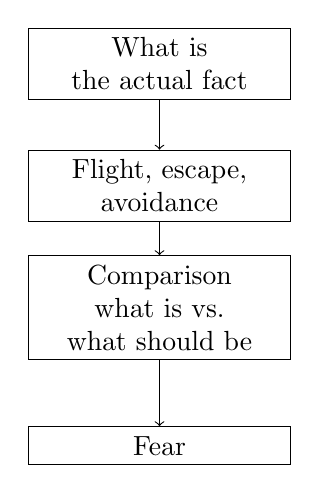
\begin{tikzpicture}
\node[draw, text width=3.1cm, align=center] (a) at (0,0) {What is\\the actual fact};
\node[draw, text width=3.1cm, align=center] (b) at (0,-1.55) {Flight, escape,\\avoidance};
\node[draw, text width=3.1cm, align=center] (c) at (0,-3.10) {Comparison\\what is vs.\\what should be};
\node[draw, text width=3.1cm, align=center] (d) at (0,-4.85) {Fear};
\draw[->] (a) -- (b);
\draw[->] (b) -- (c);
\draw[->] (c) -- (d);
\end{tikzpicture}
\caption{Transcript-based reconstruction: fear is approached as movement away from what is.}
\end{figure}

\section{Will, Analysis, And Dreams}

After the structural turn, Krishnamurti tests the familiar instruments. The first is will. The mind says, ``I will not be afraid.'' But that assertion is itself a movement against fear. It opposes fear without understanding it. Therefore, for this inquiry, the act of will has no meaning.

The lecture then becomes sharper. There are conscious fears, which one may recognise, and hidden fears, which are not immediately exposed. How are these hidden fears to be opened up? This is a natural local obstacle, and it deserves to remain in the chapter as a question rather than be flattened into a summary.

\subsection{Question \& Answer}

\paragraph{Question.} If there are hidden fears as well as conscious fears, can they be exposed through analysis? Will analysis free the mind from fear?

\paragraph{Answer.} Krishnamurti's answer is no. Analysis implies time, and time is already one of the central movements in fear. Analysis also implies an analyser. But the analyser is not outside the field being analysed. It is a fragment among the many fragments that make up the ``me,'' the ``I,'' the ego. It assumes authority over fear, while itself belonging to the same conditioned movement.

The analytic structure may be recorded as

\begin{equation}
\text{analysis}
\;\longrightarrow\;
\text{time} + \text{analyser} + \text{division}.
\end{equation}

The conclusion follows:

\begin{equation}
\text{analysis}
\;\not\longrightarrow\;
\text{ending of fear}.
\end{equation}

The deeper point is not just that analysis is slow. It is that analysis divides the analyser from the analysed. It creates a centre that will examine, judge, and evaluate fear. But that centre is already part of the same field.

\begin{proof}
The lecture's reasoning can be laid out step by step.
\begin{enumerate}
\item Hidden fear appears to require exposure.
\item Analysis proposes to expose fear by examining causes.
\item Analysis requires time, perhaps years or even a whole life.
\item Analysis also requires an analyser.
\item The analyser is not independent; it is a fragment of the conditioned ``me.''
\item The analyser separates itself from fear and treats fear as an object.
\item That separation is division.
\item Division sustains conflict and therefore does not end fear.
\end{enumerate}
Thus analysis, in this inquiry, cannot be the way to the ending of fear.
\end{proof}

Once analysis is set aside, the lecture asks whether dreams might reveal the hidden layers. But dreams too are rejected as a privileged route. They are described as the continuation of waking hours: action, doing, happening. They belong to the same movement, and so they cannot stand outside it.

\begin{table}
\centering
\begin{tabular}{p{0.27\linewidth} p{0.58\linewidth}}
Route & Why it fails in this inquiry \\
Will & It opposes fear without understanding the structure of fear. \\
Analysis & It implies time, an analyser, and division. \\
Dreams & They continue the movement of waking hours. \\
Progressive change & It postpones ending and keeps fear within time. \\
\end{tabular}
\caption{Rejected routes, kept to the terms of the lecture.}
\end{table}

This is the lecture's negative work. But it is not merely destructive. By eliminating the accustomed means, the mind becomes sensitive. The inquiry has cleared away will, analysis, dreams, and progressive time so that fear can be looked at directly.

\section{Thought, Memory, Pleasure, And Fear}

With the customary routes set aside, Krishnamurti asks again: what is fear, and how does it come? Fear is always in relation to something. It does not exist by itself. It is related to what happened yesterday, to the repetition of that tomorrow, to the memory of pain and the desire not to have that pain again.

This is the cleanest worked example in the lecture. There was pain yesterday. There is memory of it. Thought returns to that memory and projects the possibility of its repetition. The projection is fear.

\begin{align}
\text{past pain}
&\longrightarrow \text{memory} \\
&\longrightarrow \text{thought of repetition} \\
&\longrightarrow \text{fear of tomorrow}.
\end{align}

\paragraph{Example.} Let the fact be simple: there was pain yesterday. If the fact ended there, there would be the memory of an event but no psychological movement of fear. Fear enters when thought takes that memory and projects it forward: ``It may happen again.'' The mind is no longer with the fact of past pain. It is living with an image of repetition. That image is the bridge from memory to fear.

This is why the lecture says that thought brings about fear. But the next step is crucial: thought also cultivates pleasure. The inquiry cannot understand fear while treating pleasure as separate. Pleasure and fear are interrelated because thought sustains both. One cannot say, ``I will keep pleasure and have no fear.''

The pleasure chain mirrors the pain chain:

\begin{align}
\text{past pleasure}
&\longrightarrow \text{image or thought} \\
&\longrightarrow \text{desire for repetition} \\
&\longrightarrow \text{fear of loss or frustration}.
\end{align}

In the pain chain, thought projects the return of pain. In the pleasure chain, thought projects the return of pleasure. In both cases, thought carries yesterday into tomorrow, and fear enters through time.

\begin{figure}
\centering
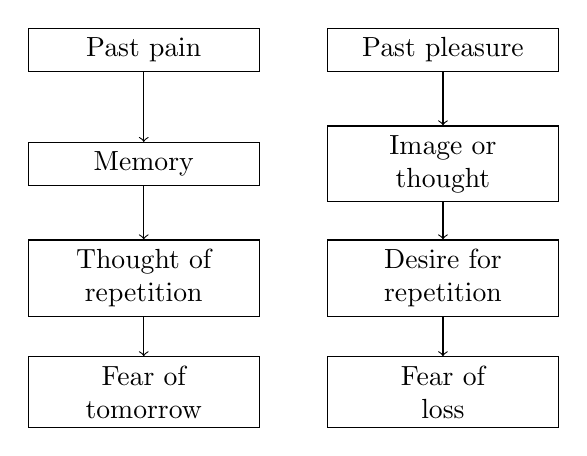
\begin{tikzpicture}
\node[draw, text width=2.7cm, align=center] (p1) at (-1.9,0) {Past pain};
\node[draw, text width=2.7cm, align=center] (p2) at (-1.9,-1.45) {Memory};
\node[draw, text width=2.7cm, align=center] (p3) at (-1.9,-2.90) {Thought of\\repetition};
\node[draw, text width=2.7cm, align=center] (p4) at (-1.9,-4.35) {Fear of\\tomorrow};

\node[draw, text width=2.7cm, align=center] (q1) at (1.9,0) {Past pleasure};
\node[draw, text width=2.7cm, align=center] (q2) at (1.9,-1.45) {Image or\\thought};
\node[draw, text width=2.7cm, align=center] (q3) at (1.9,-2.90) {Desire for\\repetition};
\node[draw, text width=2.7cm, align=center] (q4) at (1.9,-4.35) {Fear of\\loss};

\draw[->] (p1) -- (p2);
\draw[->] (p2) -- (p3);
\draw[->] (p3) -- (p4);

\draw[->] (q1) -- (q2);
\draw[->] (q2) -- (q3);
\draw[->] (q3) -- (q4);
\end{tikzpicture}
\caption{Transcript-based reconstruction: thought sustains both fear and pleasure through memory, image, and projection.}
\end{figure}

The lecture then separates joy from pleasure. Pleasure can be cultivated. It can be repeated in thought, enjoyed again through image, pursued again tomorrow. Joy cannot be treated that way. The moment thought tries to hold joy and repeat it, it has become a pleasure remembered and therefore something one is afraid to lose.

So the chapter should keep the distinction explicit:

\begin{equation}
\text{joy} \neq \text{pleasure}.
\end{equation}

More precisely,

\begin{equation}
\text{pleasure is sustained by thought},
\qquad
\text{joy is not the product of thought}.
\end{equation}

This is one of the lecture's important contributions to the larger happiness inquiry. Pleasure, fear, image, memory, and thought form a circuit. Joy is not the product of that circuit.

\section{The Difficulty Of Thought}

The lecture now reaches its central difficulty. If thought is responsible for this whole movement, what is one to do? Thought has refused to examine hidden fears, set up the analyser apart from the analysed, brought in time as a means of escaping fear while sustaining fear, and nourished pleasure. Thought is implicated in pleasure, pain, and fear.

But thought cannot simply be killed, destroyed, forgotten, or resisted. If the mind resists thought, that resistance is another movement of thought. And thought is necessary. Memory is needed to speak, to work, to go home, to function technologically, to earn a livelihood.

The fact has two sides:

\begin{align}
\text{thought} &\longrightarrow \text{practical function},\\
\text{thought} &\longrightarrow \text{psychological fear}.
\end{align}

The lecture does not solve this by suppressing one side. It asks us to see both together. Thought must function sanely and efficiently in one direction, and yet that very thought becomes a danger when it moves psychologically through memory, image, and projection.

\subsection{Question \& Answer}

\paragraph{Question.} If thought is necessary for daily functioning, and yet thought breeds fear, what is the mind to do?

\paragraph{Answer.} Krishnamurti does not answer with a method. He first asks what is the state of the mind that has gone through the inquiry. Has it actually observed the facts of analysis, time, escape, dependency, comparison, pleasure, and fear? If it has not taken the journey, it has no answer. If it has gone step by step, then the mind has become sensitive, alive, and intelligent by throwing off the burdens it had accumulated.

This pause is not decorative. It prevents the inquiry from becoming another formula. The answer depends on the quality of the mind that asks the question. A mind still seeking a technique will turn even attention into a method. A mind that has seen the facts can look at the whole process of thinking without immediately moving to suppress, justify, or escape it.

\section{The Centre, Naming, And Division}

The final movement asks whether there is a centre from which one thinks. This centre is the censor: the one who judges, evaluates, condemns, and justifies. Krishnamurti identifies it as the ``me'': my opinions, my country, my experience, my house, my family, my beliefs. From that centre, we act and think.

The centre divides. It creates opposition between my opinion and another's opinion, my country and your country, my experience and yours. If the mind observes fear from that centre, it is still caught in fear, because the centre has already separated itself from the thing it calls fear. It then says, ``I must get rid of it,'' ``I must analyse it,'' ``I must overcome it,'' ``I must resist it.'' That movement strengthens fear.

\begin{equation}
\text{centre/me}
\longrightarrow
\text{division}
\longrightarrow
\text{conflict and resistance}
\longrightarrow
\text{fear strengthened}.
\end{equation}

Naming belongs to the same movement. When fear arises and the mind says ``fear,'' the name has already brought in the past. The name is memory. It divides the observer from what is being observed. The mind is then dealing not simply with the arising fact, but with the named thing and all the accumulated reaction around that name.

\begin{equation}
\text{naming}
\longrightarrow
\text{past} + \text{division}.
\end{equation}

So the final question is precise: can the mind look at fear without the centre, and can it look without naming? That question gathers the whole lecture. Without the centre, there is no observer standing apart from fear in order to conquer it. Without naming, the mind does not immediately push the fact into the past. Observation is then no longer the old movement of division.

\begin{figure}
\centering
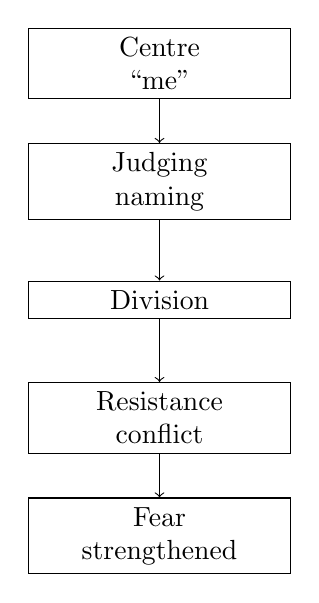
\begin{tikzpicture}
\node[draw, text width=3.1cm, align=center] (a) at (0,0) {Centre\\``me''};
\node[draw, text width=3.1cm, align=center] (b) at (0,-1.5) {Judging\\naming};
\node[draw, text width=3.1cm, align=center] (c) at (0,-3.0) {Division};
\node[draw, text width=3.1cm, align=center] (d) at (0,-4.5) {Resistance\\conflict};
\node[draw, text width=3.1cm, align=center] (e) at (0,-6.0) {Fear\\strengthened};
\draw[->] (a) -- (b);
\draw[->] (b) -- (c);
\draw[->] (c) -- (d);
\draw[->] (d) -- (e);
\end{tikzpicture}
\caption{Transcript-based reconstruction: the centre strengthens fear by dividing itself from what it calls fear.}
\end{figure}

The alternative is stated cautiously:

\begin{equation}
\text{observation without centre and without naming}
\longrightarrow
\text{ending of fear}.
\end{equation}

This arrow should not be read as a mechanical technique. It records the lecture's conclusion: when the mind observes closely, with care, affection, and attention, and without the accustomed division of a centre, there is an ending of fear, hidden and open.

\section{Summary}

The lecture moves in a deliberate sequence. It begins by showing why fear matters: fear obstructs seriousness, enjoyment, and joy. It then establishes the condition of inquiry: communication as shared attention rather than agreement, disagreement, or comparison.

From there, Krishnamurti surveys the many forms of fear and turns from particular instances to structure. Fear is watched as movement away from what is, and comparison is one of its central forms. The customary answers are then set aside. Will is another movement against fear. Analysis implies time, an analyser, and division. Dreams continue the movement of waking life.

Only after that clearing does the lecture turn to thought. Thought, through memory and projection, produces fear from past pain and sustains pleasure through image and repetition. Pleasure and fear are therefore interrelated, while joy is distinguished from both because it is not the product of thought.

The final movement concerns the centre. The ``me'' divides itself from fear, names it, judges it, resists it, and thereby strengthens it. The ending of fear is not presented as suppression or method, but as direct observation without the centre and without naming. In that attention, the lecture says, fear can end.